% Created 2025-03-29 Sat 16:03
% Intended LaTeX compiler: pdflatex
\documentclass[11pt]{article}
\usepackage[utf8]{inputenc}
\usepackage[T1]{fontenc}
\usepackage{graphicx}
\usepackage{longtable}
\usepackage{wrapfig}
\usepackage{rotating}
\usepackage[normalem]{ulem}
\usepackage{amsmath}
\usepackage{amssymb}
\usepackage{capt-of}
\usepackage{hyperref}
\author{Jackson Mowry}
\date{\today}
\title{Report}
\hypersetup{
 pdfauthor={Jackson Mowry},
 pdftitle={Report},
 pdfkeywords={},
 pdfsubject={},
 pdfcreator={Emacs 30.1 (Org mode 9.7.11)}, 
 pdflang={English}}
\begin{document}

\maketitle
\tableofcontents

\section{Part 1 -- Investigating Web PKI Certificates}
\label{sec:org64de6df}
\subsection{google.com}
\label{sec:org95df4dd}
\begin{enumerate}
\item What is the subject of the leaf certificate?
\begin{itemize}
\item *.google.com
\end{itemize}
\item What is the issuer of the leaf certificate?
\begin{itemize}
\item WR2, \url{http://i.pki.goog/wr2.crt}
\end{itemize}
\item What is its validity period?
\begin{itemize}
\item 10 Mar 2025 - 2 Jun 2025
\end{itemize}
\item What type of public key is it using?
\begin{itemize}
\item EC 256 Bits
\end{itemize}
\item What algorithm was used to sign the certificate?
\begin{itemize}
\item SHA256withRSA
\end{itemize}
\end{enumerate}
\subsection{amazon.com}
\label{sec:orgef704e2}
\begin{enumerate}
\item What is the subject of the leaf certificate?
\begin{itemize}
\item *.peg.a2z.com
\end{itemize}
\item What is the issuer of the leaf certificate?
\begin{itemize}
\item DigiCert Global CA G2
\end{itemize}
\item What is its validity period?
\begin{itemize}
\item 26 Aug 2024 - 27 Jul 2025
\end{itemize}
\item What type of public key is it using?
\begin{itemize}
\item RSA 2048 Bits
\end{itemize}
\item What algorithm was used to sign the certificate?
\begin{itemize}
\item SHA256withRSA
\end{itemize}
\end{enumerate}
\subsection{utk.edu}
\label{sec:orgce8069e}
\begin{enumerate}
\item What is the subject of the leaf certificate?
\begin{itemize}
\item utk.edu
\end{itemize}
\item What is the issuer of the leaf certificate?
\begin{itemize}
\item R10
\end{itemize}
\item What is its validity period?
\begin{itemize}
\item 5 Mar 2025 - 3 Jun 2025
\end{itemize}
\item What type of public key is it using?
\begin{itemize}
\item RSA 2048 Bits
\end{itemize}
\item What algorithm was used to sign the certificate?
\begin{itemize}
\item SHA256withRSA
\end{itemize}
\end{enumerate}
\subsection{dhs.gov}
\label{sec:org986025b}
\begin{enumerate}
\item What is the subject of the leaf certificate?
\begin{itemize}
\item www.dhs.gov
\end{itemize}
\item What is the issuer of the leaf certificate?
\begin{itemize}
\item GeoTrust RSA CA 2018
\end{itemize}
\item What is its validity period?
\begin{itemize}
\item 29 Jan 2025 - 16 Dec 2025
\end{itemize}
\item What type of public key is it using?
\begin{itemize}
\item RSA 2048 Bits
\end{itemize}
\item What algorithm was used to sign the certificate?
\begin{itemize}
\item SHA256withRSA
\end{itemize}
\end{enumerate}
\subsection{self-signed.badssl.com}
\label{sec:org3da28cc}
\begin{enumerate}
\item What is the subject of the leaf certificate?
\begin{itemize}
\item *.badssl.com
\end{itemize}
\item What is the issuer of the leaf certificate?
\begin{itemize}
\item *.badssl.com (Self-signed)
\end{itemize}
\item What is its validity period?
\begin{itemize}
\item 25 Mar 2025 - 25 Mar 2027
\end{itemize}
\item What type of public key is it using?
\begin{itemize}
\item RSA 2048 Bits
\end{itemize}
\item What algorithm was used to sign the certificate?
\begin{itemize}
\item SHA256withRSA
\end{itemize}
\item Problematic Field?
\begin{itemize}
\item Issue, to fix this you would need to get a certificate signed by a trusted CA, not signed by the subject itself.
\end{itemize}
\end{enumerate}
\subsection{untrusted-root.badssl.com}
\label{sec:org87883ff}
\begin{enumerate}
\item What is the subject of the leaf certificate?
\begin{itemize}
\item *.badssl.com
\end{itemize}
\item What is the issuer of the leaf certificate?
\begin{itemize}
\item BadSSL Untrusted Root Certificate Authority
\end{itemize}
\item What is its validity period?
\begin{itemize}
\item 25 Mar 2025 - 25 Mar 2027
\end{itemize}
\item What type of public key is it using?
\begin{itemize}
\item RSA 2048 Bits
\end{itemize}
\item What algorithm was used to sign the certificate?
\begin{itemize}
\item SHA256withRSA
\end{itemize}
\item Problematic Field?
\begin{itemize}
\item Issuer, this issue is not in our browsers trust store. We would need to get our certificate request signed by a commonly trusted CA.
\end{itemize}
\end{enumerate}
\subsection{wrong.host.badssl.com}
\label{sec:org982449d}
\begin{enumerate}
\item What is the subject of the leaf certificate?
\begin{itemize}
\item badssl-fallback-unknown-subdomain-or-no-sni
\end{itemize}
\item What is the issuer of the leaf certificate?
\begin{itemize}
\item BadSSL Intermediate Certificate Authority
\end{itemize}
\item What is its validity period?
\begin{itemize}
\item 8 Aug 2016 - 8 Aug 2018
\end{itemize}
\item What type of public key is it using?
\begin{itemize}
\item RSA 2048 Bits
\end{itemize}
\item What algorithm was used to sign the certificate?
\begin{itemize}
\item SHA256withRSA
\end{itemize}
\item Problematic Field?
\begin{itemize}
\item Subject, this does not match the actual domain of the site. We would need to get a certificate that is explicitly bound to the domain.
\item Additionally the certificate is also expired, therefore we would need to get a new certificate.
\end{itemize}
\end{enumerate}
\subsection{expired.badssl.com}
\label{sec:org8a04477}
\begin{enumerate}
\item What is the subject of the leaf certificate?
\begin{itemize}
\item *.badssl.com
\end{itemize}
\item What is the issuer of the leaf certificate?
\begin{itemize}
\item COMODO RSA Domain Validation Secure Server CA
\end{itemize}
\item What is its validity period?
\begin{itemize}
\item 9 Apr 2015 - 12 Apr 2015
\end{itemize}
\item What type of public key is it using?
\begin{itemize}
\item RSA 2048 Bits
\end{itemize}
\item What algorithm was used to sign the certificate?
\begin{itemize}
\item SHA256withRSA
\end{itemize}
\item Problematic Field?
\begin{itemize}
\item Valid until, this certificate expired almost 10 years ago. To fix this we would need to get another certificate.
\end{itemize}
\end{enumerate}
\section{Part 2 -- Using an Email PKI Certificate}
\label{sec:orgdc4fb58}
\begin{enumerate}
\item The name of the student with which you (attempted to) exchanged secure email.
\begin{itemize}
\item Peter (MACk Address) Hansen
\end{itemize}
\item What was the process for creating a certificate?
\begin{itemize}
\item We first tried to create our own self-signed certificates follwing this online guide, \url{https://community.lansweeper.com/t5/quick-tech-solutions/how-to-sign-an-email-with-a-self-signed-s-mime-certificate/ba-p/62255}. That ended up being a dead-end as we could not find an easy way to trust self-signed certificates in Thunderbird. After that we found an online service named Actalis which was very frustrating to use. In the end we don't think we were doing anything wrong, their service just suddenly emailed us the necessary information around 3 hours after we originally requested it. From there it was as simple as downloading our .p12 file and unlocking it with the password provided to us.
\end{itemize}
\item What was the process for getting that certificate signed?
\begin{itemize}
\item Once we requested a certificate from Actalis we realized that they would generated the CSR for you, meaning the generation and signing was all handled on their end. This basically involved waiting around 3 hours for the request to be processed.
\end{itemize}
\item What was the process for sharing a key between you and your partner?
\begin{itemize}
\item The process of sharing the key was not immediately obvious and we first tried to manually import each other's .p12 key into Thunderbird. We then realized this process was probably incorrect as it involved having to also share the associated password just to import it. Additionally, Thunderbird was not allowing us to import the .p12 file through the associated screen. Eventually we read online that you can first send a digitally signed email, which will automatically distribute your public key to the recipient. This then allowed the recipient to respond with an encrypted email, then finally the original sender is allowed to send an encrypted message back. This is fairly nice as only 1 message has to be sent unencrypted before encrypted communication can begin.
\end{itemize}
\item Include a screenshot of the signed and encrypted email you send and the email you received.
\begin{center}
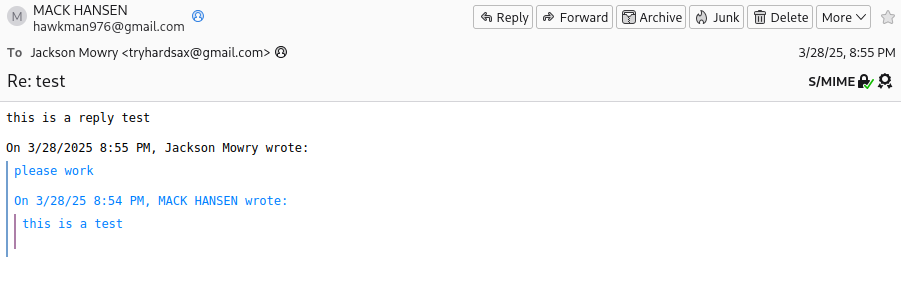
\includegraphics[width=.9\linewidth]{screenshot-1743277577_901x297.png}
\end{center}
\begin{center}
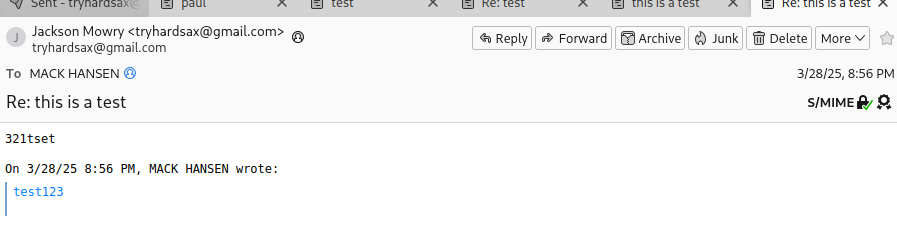
\includegraphics[width=.9\linewidth]{screenshot-1743277613_897x242.png}
\end{center}
\begin{center}
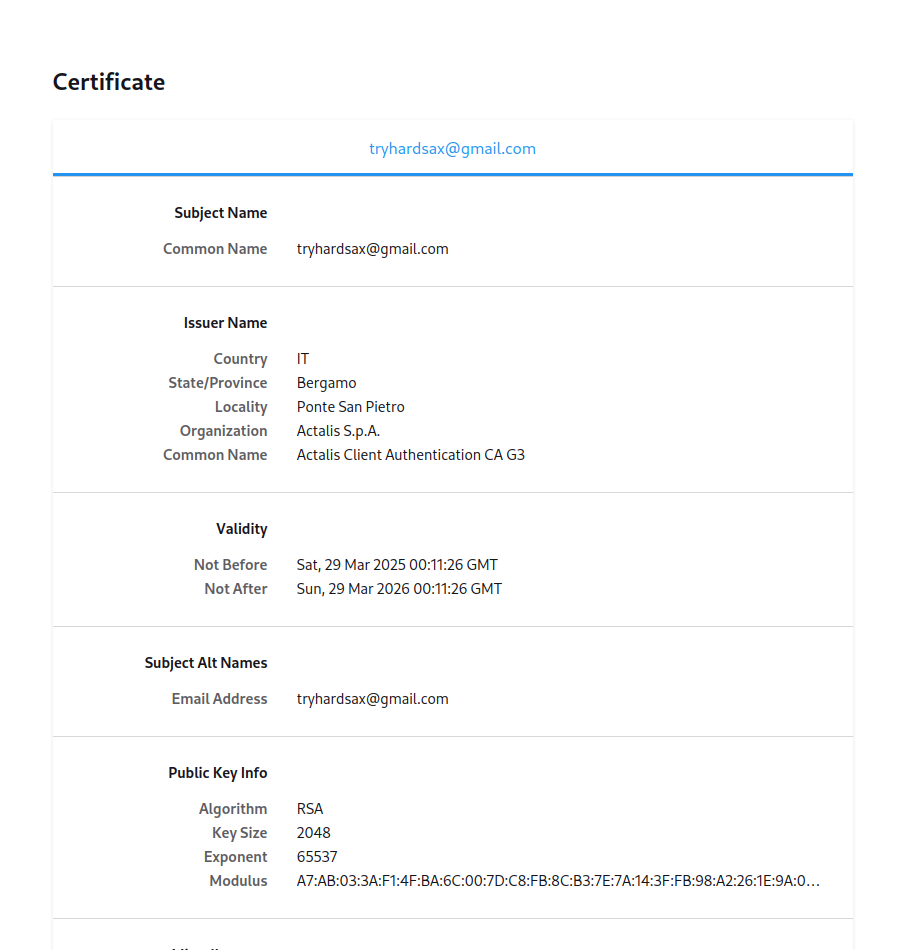
\includegraphics[width=.9\linewidth]{screenshot-1743277622_903x950.png}
\end{center}
\begin{center}
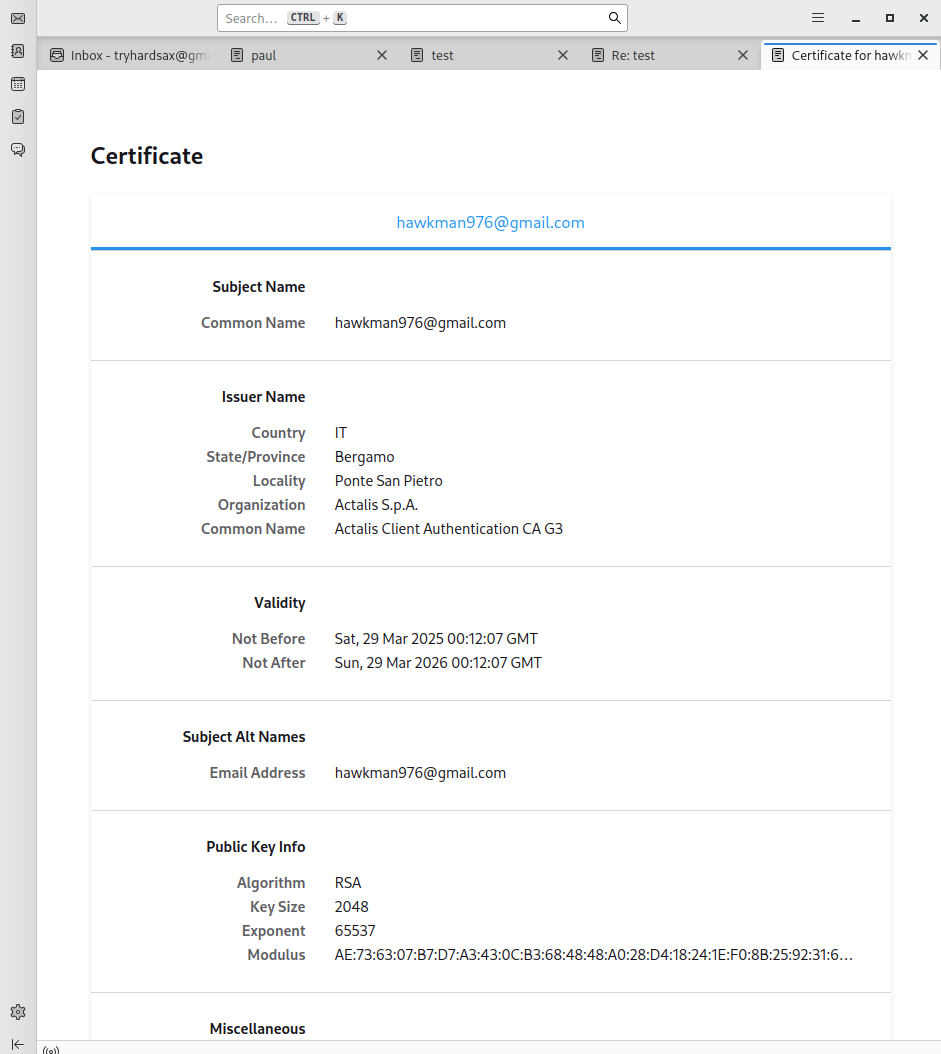
\includegraphics[width=.9\linewidth]{screenshot-1743277560_941x1054.png}
\end{center}
\begin{enumerate}
\item Identify where in the images you were able to verify the signature.
\begin{itemize}
\item The small 'ribon' icon has a pop-out menu that shows both encryption and digital signatures were used the messaged, sadly I cannot both open the menu and take a screenshot, but hopefully you get the idea. This is present on both my sent and received message.
\end{itemize}
\item Identify where in the image you were able to confirm that encryption was used.
\begin{itemize}
\item Encryption was found in the 'ribon' menu I mentioned before, additionally within that menu you can see the actual certificate used by the send, which I have included summary screenshots for both me and my partner.
\end{itemize}
\end{enumerate}
\item Explain which parts of the process were difficult to understand or execute.
\begin{itemize}
\item The only real difficult part was finding information about the topic. Once we learned what to do the actual process was painless. For us the overall hardest part was just sitting around waiting for the certificate. During this time we were trying various different methods to obtain another certificate, which ultimately came up short. Lastly, it was not clear to us that our partner's certificate would be automatically imported after sending a digitally-signed email, before we would be allowed to encrypt an email.
\end{itemize}
\item Rate your experience using the System Usability Scale . Give your answer for each question and compute your overall score.
\begin{enumerate}
\item I think that I would like to use this system frequently.
\begin{itemize}
\item 5. I would, just because I highly value confidentially and integrity.
\end{itemize}
\item I found the system unnecessarily complex.
\begin{itemize}
\item 4. Yes, there were certainly parts that could have been made much more obvious to users.
\end{itemize}
\item I thought the system was easy to use.
\begin{itemize}
\item 4. Once we got through the setup the actual using of the system was easy.
\end{itemize}
\item I think that I would need the support of a technical person to be able to use this system.
\begin{itemize}
\item 1. No, I think this would work fairly easily going forward.
\end{itemize}
\item I found the various functions in this system were well integrated.
\begin{itemize}
\item 3. If we're including the processing of getting the certificate then I could say no, otherwise yes.
\end{itemize}
\item I thought there was too much inconsistency in this system.
\begin{itemize}
\item 1. The system felt very consistent.
\end{itemize}
\item I would imagine that most people would learn to use this system very quickly.
\begin{itemize}
\item 1. Most users would have no hope of using this system.
\end{itemize}
\item I found the system very cumbersome to use.
\begin{itemize}
\item 1. Now that I understand it I think it works fairly well.
\end{itemize}
\item I felt very confident using the system.
\begin{itemize}
\item 5. Now that I understand the system I would agree.
\end{itemize}
\item I needed to learn a lot of things before I could get going with this system.
\begin{itemize}
\item 4. This is true, the concept of certificates on a person-by-person level is new to me.
\end{itemize}
\end{enumerate}
\item Total Score
\begin{itemize}
\item 67.5, which is just below a C.
\end{itemize}
\item Now that you know about secure email technology, will you continue using it in the future? Why or why not?
\begin{itemize}
\item I think that the biggest problem in my social circle would be adoption. If the process was similar to PGP email encryption I think I would have a much higher chance at success.
\end{itemize}
\end{enumerate}
\end{document}
